%!TEX root = proceedings.tex
\section{Emergent Themes}
We identified several aspects of the on-demand markets we studied that seem to apply in generalizable ways.
These characteristics and issues extend beyond the more narrowly scoped issues of scheduling workers and handling payments which might seem more at the focal point of designing a labor market, although those issues too must be addressed;
we focus specifically on the social negotiations that a technological system must broker.
These guidelines are illustrated using mock-ups and a mobile application front-end developed in tandem with organization C, organization B, \& organization E, and consist of the following considerations:

\begin{enumerate} \itemsep0pt \parskip0pt
  \item Constructive feedback
  \item Assigning work fairly
  \item Managing customer expectations
  \item Protecting vulnerable workers
  \item Reconciling worker identities
  \item Assessing worker qualifications
  \item Communicating worker quality
% \item Feedback
% \item Assigning Work
% \item Customer Expectations
% \item Vulnerable Workers
% \item Worker Identity
% \item Worker Qualifications
% \item Worker Quality \& Ratings
\end{enumerate}


\subsection{1.        Constructive Feedback}
%!TEX root = ../proceedings.tex
% \subsection{Feedback}
\textit{Ratings cause anxiety, whereas feedback can satisfy the same administrative needs without causing workers undue stress.}

At organization E, we learned that workers interpreted negative feedback very personally,
making it difficult for them to internalize that feedback constructively and act on the suggestions customers made.
Multiple issues may have been at play here;
cultural differences might explain a mismatch in how feedback is offered and how it is received,
but so too would the power imbalance between undocumented domestic workers and their customers.

organization E didn't seem to investigate the cause of this effect,
but their solution circumvented this problem entirely.
Rather than giving workers unfiltered, raw feedback as it streamed in,
organization E intercepted reviews from customers and distilled them into constructive, actionable feedback.
Both praise and criticism would sometimes be read aloud to the entire group,
with identifying information removed.

\begin{figure}[t]
\centering
  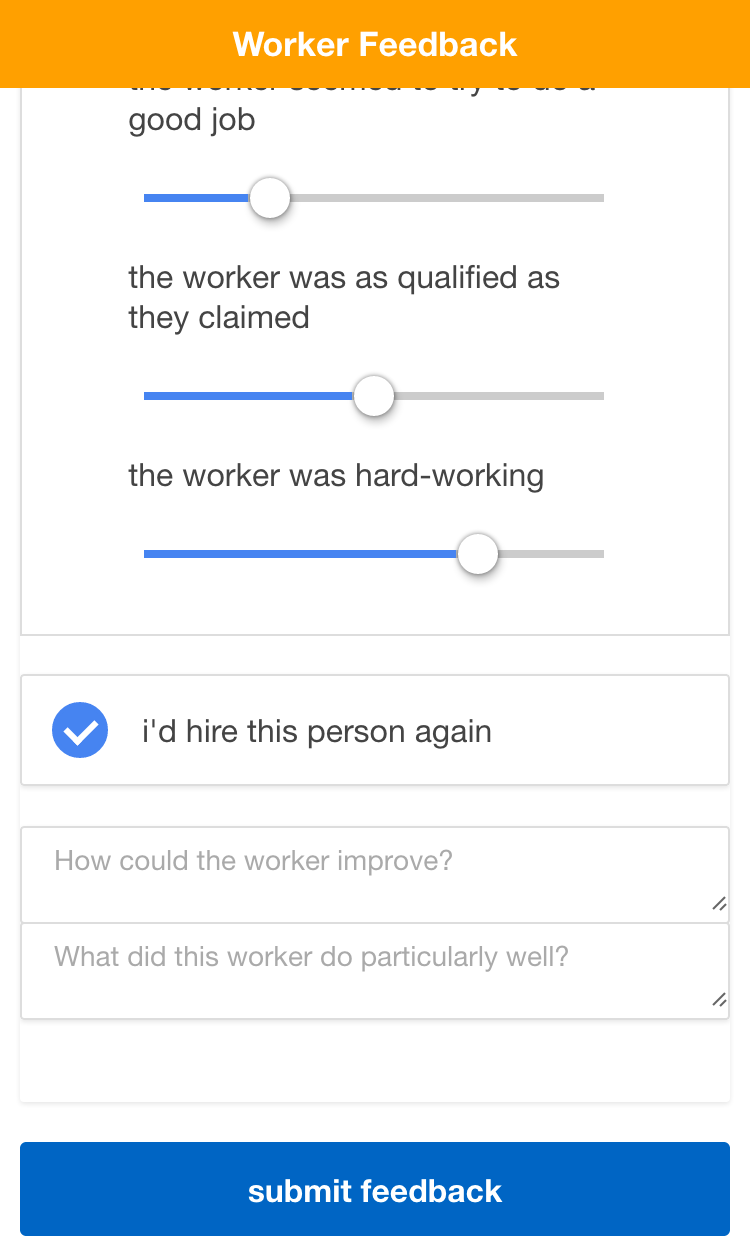
\includegraphics[width=1\columnwidth]{figures/feedback}
    \caption{Given quantitative prompts and qualitative follow-up questions,
  research suggests that users are more likely to write more,
  which can better-inform.}~\label{fig:workerFeedback}
\end{figure}

The purpose of reading positive feedback publicly was to reaffirm the group's sense of worth in a shared sense of success;
the purpose of reading the negative feedback, meanwhile, was to prompt workers to reflect on what went ``wrong'', and how to avoid such an outcome in the future.
A shared sense of failure also seemed to affect workers in these cases;
whether this is an outcome of public readings of reviews, or more complex relationships between workers and organization E, is unclear.

Speaking with Uber and Lyft drivers, we found an alternative approach to providing workers with feedback;
drivers are made aware of an aggregated rating
--- generally a moving average of the previous \textit{n} ratings ---
but they are not exposed to qualitative feedback in any form, even when customers provide it.

A driver's current aggregated rating, it turns out, is extremely important:
a driver's rating determines the worker's eligibility to do work, and falling below various thresholds carries various consequences. Reports suggesting that these thresholds are finely tuned as well as closely guarded secrets make these markets particularly emotionally taxing for workers \cite{leakedUber}.

When we spoke to drivers, they relayed stories of apparent obligations to take expensive remedial courses if their overall rating dropped below a certain threshold,
and widely held fears of suspension and deactivation for falling below an unknown level weigh heavily on workers' minds.
Frustration directed at drunk, clumsy, or naive passengers accidentally or deliberately giving drivers a rating of 4 (out of 5) stars further exacerbates stress.

Markets which aim to empower ``gig workers'' should use quantitative rating systems sparingly,
or to prompt more detailed qualitative feedback, as we illustrate in Figure
\ref{fig:workerFeedback}.
Quantitative ratings in the form of Likert scales followed by qualitative prompts for feedback seem to precipitate more detailed feedback
\cite{numericCritique}.

% While quantitative metrics
% --- like approval rates and moving average ratings ---
% make large-scale evaluation seemingly manageable and generalizable,
% the professional stress these
Quantitative metrics --- especially those that are opaquely evaluated --- do not benefit workers, nor does it seem they even inform appropriate customer behavior \cite{ebayRatings}.
Meanwhile, constructive feedback suggesting improvements may provide workers with the necessary information to improve as professionals without causing undue stress over issues such as worker eligibility..
\subsection{2.        Assigning Work Fairly}
%!TEX root = ../proceedings.tex
% \subsection{Assigning Work}
\textit{Who gets new work opportunities first is a contentious issue which should be negotiated by people, enforced by technology.}

When new work becomes available, who should have first access to claim it proves to be a contentious topic.
Depending on the intended velocity of the market, various suggestions have emerged.

In existing technologically enabled markets, we find some of these decisions have been made carefully.
Some of these approaches are worth considering, and can be described thusly:
\begin{itemize} \itemsep0pt \parskip0pt
  \item On AMT, Turkers find themselves in constant competition with one another to claim HITs;
  the effects of this task searching behavior have been explored in some detail \cite{taskSearch}.
  \item Airbnb, Craigslist, and others invite workers to describe the services or products they offer, and leave the work of matching to customers.
  The complex nature of finding a suitable place to live may make this approach preferable over automated matching.
  \item Uber, Lyft, and others use algorithmic matching to determine who should be offered work;
  it is unclear to workers and consumers who is given a job offer first,
  but drivers we spoke to assumed that the nearest drivers were given first offer of a new job in markets such as Uber \& Lyft.
\end{itemize}

Among each of these approaches designers can make choices that dramatically affect the experiences for workers and customers.
The first option, used by Amazon Mechanical Turk, Craigslist, etc\dots makes it possible for job turnover to be extremely high, but the cost is that workers may feel stressed by the uncertainty over whether a job they're considering has already been claimed.
The second approach mentioned, which Airbnb uses, gives customers the choice to contact ``workers", but the process of finding a provider makes the overall matching process time-consuming.

When we spoke with members of organization B and organization A,
the consensus we initially found was that seniority within a reasonable proximity to the work would be the fairest solution to the problem we described.
After some discussion, it emerged that this position was not universally shared among members of either group.
Perhaps understandably, younger members of organization B felt that workers who had been working longer that day without having been offered any jobs,
or workers who were significantly closer, should eventually be given higher priority for work.

organization E chose yet another option, primarily using a random selection process at the beginning of each hiring day by pulling the names of currently present workers out of a jug;
every eligible worker has a reasonable chance at being selected first, just as they have a chance of coming up last.
Workers could short-circuit the selection process by volunteering to do work beneficial to the group
--- for example, making coffee, or sweeping the common room's floors.
By volunteering to do this work, they're guaranteed first priority for incoming jobs the following day,
This ensures that they'll be given an offer for work quickly on the following day.

The best option for most markets might be the model Uber, Lyft, and others have adopted,
where customers are automatically routed to workers,
who are given a time window where they have exclusive claim to a job that's been posted.
If they reject a job offer, the job moves to the next eligible worker.

\begin{figure}[t]
\centering
  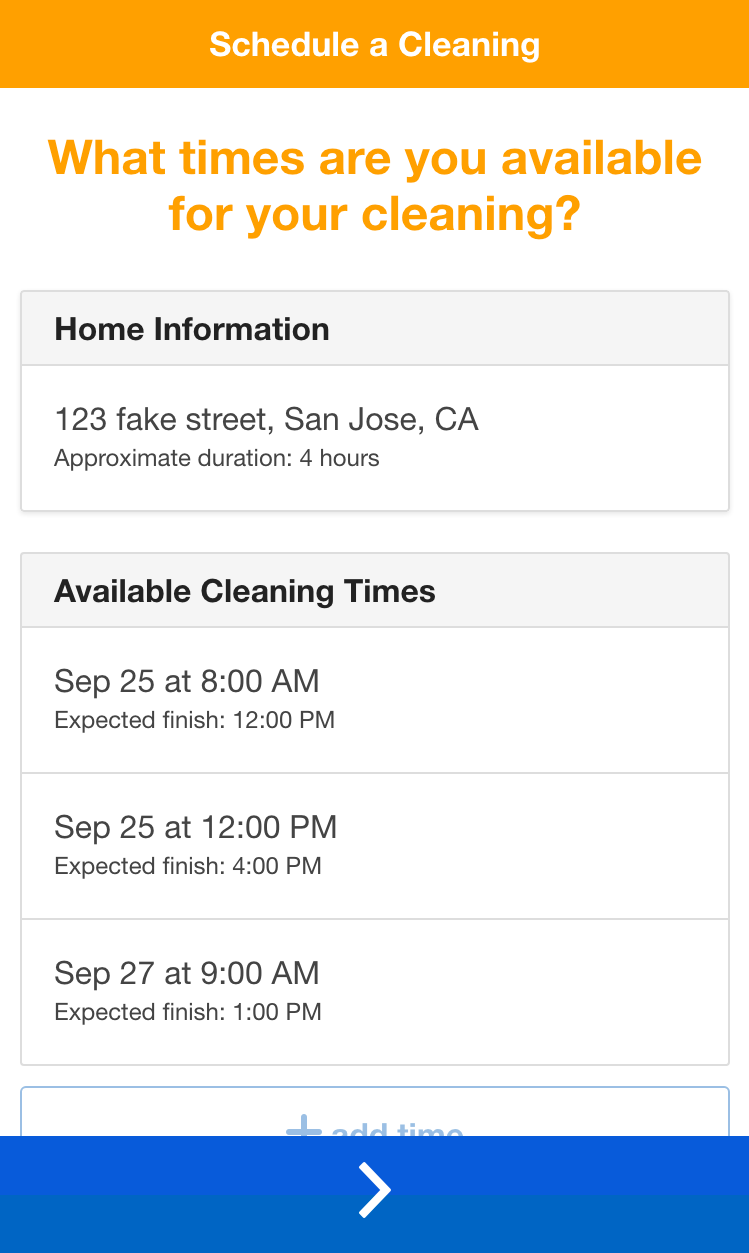
\includegraphics[width=1\columnwidth]{figures/scheduling}
    \caption{In the client's perspective, a lightweight scheduling system can suffice to communicate availability.}~\label{fig:clientSchedule}
\end{figure}
\begin{figure}[t]
\centering
  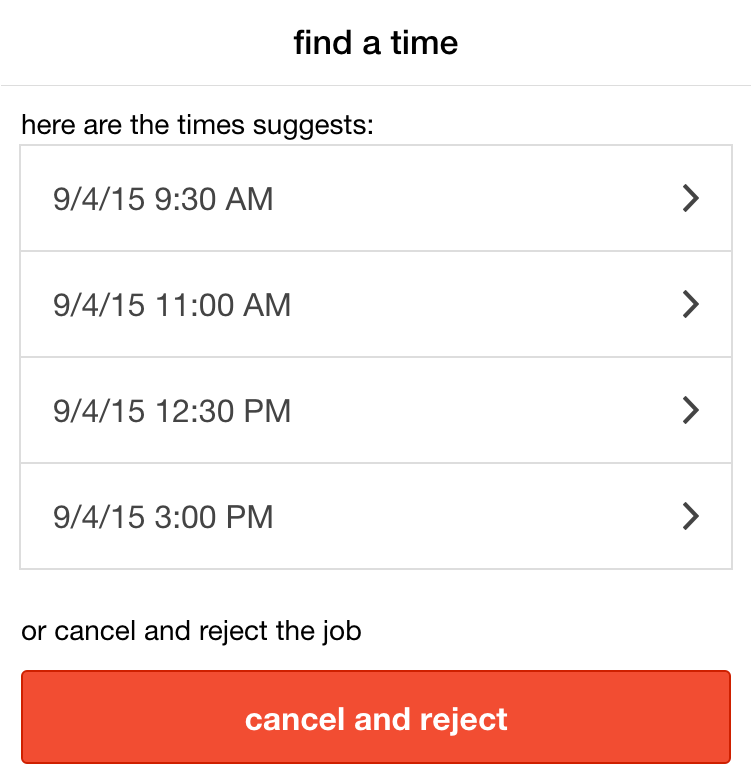
\includegraphics[width=1\columnwidth]{figures/jobtimesoffer}
    \caption{In the worker's perspective, scanning suggested start times can make scheduling easier than entering a series of windows of availability each week or month.}~\label{fig:workerSchedule}
\end{figure}

The task of finding eligible, willing workers can be simplified by considering availability,
narrowing the list of candidate workers to those who are interested in working during a given time frame.
This can, however, be a particularly frustrating challenge for on-demand workers.
One of the most common reasons we heard from gig workers who preferred such work was the flexibility that mode of work offered;
in other words, trying to get workers to commit to windows of availability goes against the nature of that work --- the freedom --- which made it appealing to those we consulted.

This challenge was ameliorated in various ways across field sites; At organization E, workers were assigned each day even if work was solicited days or weeks in advance (unless, of course, a specific worker was requested for repeat work). This process neatly handles the potentially ambiguous question of availability for a number of workers, but it's limiting in two ways:

\begin{enumerate} \itemsep0pt \parskip0pt
  \item organization E's scale is ultimately limited by their ability to process workers on a daily basis (this was particularly salient as a volunteer, processing workers as they arrived to check at 7 A.M.)
  \item Workers who wished to be available for leads had to travel to the organization E offices; sometimes workers would travel north as many as 30 minutes, only to get a job 30 minutes south again.
\end{enumerate}

Instead of setting availability in advance, we suggest optimizing the process of scheduling so that workers and customers spend a minimal amount of time negotiating one another's availability.

This leaves open the question of how that list of workers is determined;
who is the first choice, and who's second if the first worker doesn't claim the job?
Who ends up getting last pick?

We can only offer that this factor is determined in large part by the organization running the system.
A template for a worker-run marketplace should therefore expose these options,
and more importantly surface the debate at the core of these discussions,
while abstracting away the technical details such as implementation.
These cases also illustrate that systems can be designed in ways that meaningfully and fairly reward workers for doing necessary work for the benefit of the community as a whole.

\subsection{3.        Managing Customer Expectations}
%!TEX root = ../proceedings.tex
% \subsection{Customer Expectations}
\textit{Clear expectations of all participants in trade benefit all, but introducing those expectations can be difficult for all parties.}

Perhaps the most common source of dissatisfaction with gig workers comes from a miscommunication or simply a mismatch in the expectations of the customer and the worker.
The effects of this mismatch appear to have been discussed when discussing Mechanical Turk, leading to norms where ``good" requesters know to provide examples of correct work and highlight common mistakes, explicating the intent of the micro work.
On other platforms, clear expectations are established ahead of time
(on ride-sharing markets, the expected driving path, estimated time, and estimated cost is displayed to customers).

People we spoke with at organization B, organization E, and organization C felt that formalizing the expectations of workers was the most appropriate solution to this problem.
By making it clear to customers what workers are expected to do
(for instance, what specific tasks go into cleaning a kitchen),
expectations of customers are set reasonably, workers can be trained properly,
and disputes about whether the worker did the job properly or sufficiently become less ambiguous.

\begin{figure}[t]
\centering
  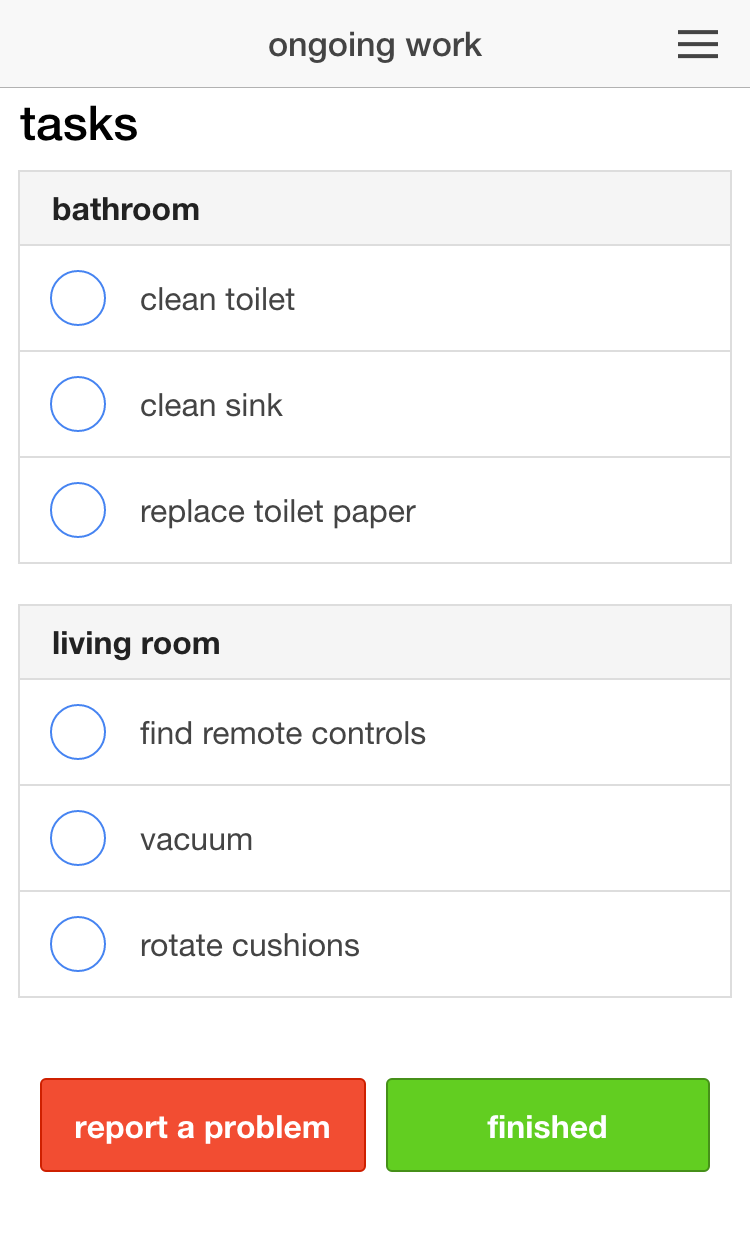
\includegraphics[width=1\columnwidth]{figures/checklist}
    \caption{Explicit checklists make it easier for workers to verify that they've completed all expected work;
    it also makes it apparent to customers that they need to add or clarify certain tasks.}~\label{fig:checklist}
\end{figure}

We tend to agree with this approach.
In our fieldwork we found that paper checklists made it clearer to customers what to expect to be done
--- and importantly, what to expect not to be done.
If customers wanted additional work completed, they could specify that and agree to the extra time it would take to do that job, which they sometimes did.

This ``contract'' between workers and customers can be written collaboratively by both parties,
outlined by the workers themselves, or directed principally by customers as they describe the work they need completed;
the exact process is less important than the shared understanding of the constituent tasks.
\subsection{4.        Protecting Vulnerable Workers}
%!TEX root = ../proceedings.tex
% \subsection{Vulnerable workers, and how to protect them}
\textit{Many workers in the gig economy are vulnerable to exploitation;
careless or malicious systems can endanger workers.}

At organization E, workers expressed concern when we discussed the ability to show a profile picture to customers in advance of their arrival.
These concerns stemmed from fears of their privacy being violated,
and discrimination over their race, age, gender, and other characteristics.
In particular, workers at organization E were afraid that customers would reject them for being too old.

organization E addressed this issue by emphasizing the qualifications of workers,
abstracting their names and details for first-time jobs.
Workers fundamentally have final say over whether to be matched to a customer,
based on general data about the location,
an indication of whether they've worked together before, and a rough estimate of the amount of work solicited
(In most cases, a precise estimate of how long a job will take is difficult to make without someone familiar with the work on-site to make an informed estimate).

If a customer has hired through organization E before and wants to hire a previously hired worker,
a rudimentary system allows volunteer dispatch staff to identify those workers for matching.
This allows workers to gradually develop a body of clients over time;
eventually, they no longer rely on organization E to refer customers to them at all.
Organization A utilized a similar approach, allowing customers to request a worker they've worked with in the past,
but otherwise not revealing information about workers to customers.

Many of the existing marketplaces for gig work don't expose such affordances to request a previously hired worker.
% making it difficult or impossible to grow a regular client base without leaving the system entirely.
This may be deliberate, as it effectively prevents workers from fostering a community of clients.
By preventing workers and customers from becoming familiar,
workers become dependent on the market created by the platform to provide leads on customers.
Whether a system promotes such dependence or not is up to the system's designers,
but we articulate a possible approach which makes repeat work possible.

As we illustrate in Figure ~\ref{fig:previousHire},
a simple interface exposing basic information about a previously hired worker can remind a customer whom they want to select.
Further, a technological solution such as this can ease the negotiation of scheduling;
in our case, we suggest prompting the worker for their availability.
Once several times are suggested, the customer can select and confirm a time.


\begin{figure}[t]
\centering
  
\includegraphics[width=1\columnwidth]{figures/recurrent}
    \caption{By exposing some information about previously matched workers,
    a system can facilitate workers developing a reliable customer base.}~\label{fig:previousHire}
\end{figure}

Working with organization B, nurses we spoke to expressed concern over disrespectful or uncooperative patients.
Nurses described various safety concerns including
violent neighborhoods, dangerous pets such as dogs, and patients in declining mental health.
Nurses told us that these were inherent risks associated with in-home care.
Some of the nurses that we spoke to clarified that, in cases where they felt a particular danger,
they may decline to meet a patient and communicate that concern later.

\begin{figure}[t]
\centering
  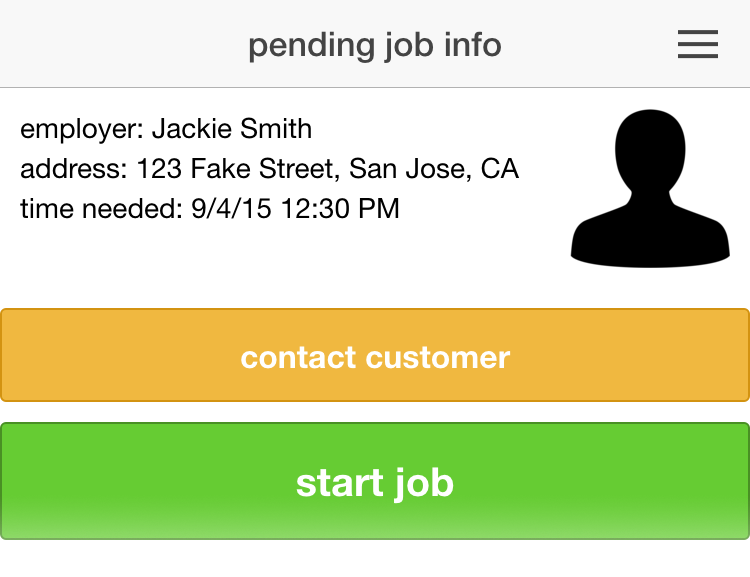
\includegraphics[width=1\columnwidth]{figures/startwork}
    \caption{A simple interface for workers,
    allowing them to contact customers,
    facilitates the resolution of potential issues before work begins,
    such as difficulty finding a location, ambiguity in instructions, etc\dots}~\label{fig:startwork}
\end{figure}

Technological systems can assist workers in cases like these;
by exposing customer contact information to workers (and potentially vice versa),
workers can contact customers before they begin work to clarify or resolve any issues.

\subsection{5.        Reconciling Worker Identities}
%!TEX root = ../proceedings.tex
% \subsection{Worker identity versus ``gig workers"}
\textit{The very features that make gig work appealing also stymie attempts to coalesce stable worker advocacy groups.}

At organization E, organization A, organization C, and organization B we observed a subtle but important characteristic;
everyone at these organizations identified primarily by the work that they did.
Members of organization E self-identified as house cleaners and day laborers;
People at organization A were workers, first and foremost.
The same fundamental sentiment was shared by nurses affiliated with organization B.

We found that this carried an important effect;
at organization E the effect was most salient that workers identified together and recognized the importance of maintaining organization E's positive reputation among customers.
Every week, organization E administrative staff would read reviews of workers,
made anonymous beforehand,
allowing the workers to reflect on these frequent successes and occasional failures.

Perhaps most surprising was a shared sense of success and failure when workers listened to this feedback;
people we spoke to felt that they had upheld or let down their peers and the organization of which they were part,
even if the review was not of their own work.
This strong sense of group identity seemed to drive workers to work hard to maintain the already good reputation that organization E enjoyed.

When we spoke to drivers in the gig economy, some told us that they had previously worked for competing yellow cab companies.
They explained that they gave up on conventional cab companies was because requirements to drive for yellow cabs felt onerous.
Drivers worked for Uber and Lyft because those markets allowed them to drive as much or, importantly, as little as they wanted.
At some yellow cab companies, a monthly fee was required for access to the cabs themselves.

This presents a potential challenge for those hoping to build communities fostering collective decision-making and action.
As Kraut et al. point out, a crucial component in designing successful online communities is identification with the group
\cite{successfulOnlineCommunities}.
This is already a difficult goal to achieve, now exacerbated by the nature of the community involved.
Features that makes gig work appealing
--- the freedom to come and go as one pleases, for instance ---
make it that much more difficult to form a shared sense of community based on shared identities.

Indeed, workers in the gig economy tended not to think of themselves as identified by the work that they do ---
many drivers, for instance, volunteered that they were musicians, security guards, and even elementary school teachers.
Their work as drivers, then, was not substantively important to who they are.
Workers at organization E, meanwhile, identified as cleaners, day laborers, etc\dots without qualification.

Among many of the ``gig workers" that we spoke to, the sense of freedom and independence turned out to be an important feature of their identity.
The relative freedom over when and indeed whether to work was, it seemed, powerfully appealing.

This represents a difficult dilemma for labor unions and other conventional worker advocacy groups,
which rely on the shared sense of identity of workers,
who are now increasingly detaching their identities from the work that they do.

We assume that a worker-centric market needs emotional investment from its participants in order to succeed,
and the evidence seems to corroborate this sense \cite{dynamo,olsonlogic,russell1982collective}.
Given this premise, it seems that workers in a system must appreciate their reliance on their group's collective success.
Balancing this need with the desire that workers have expressed to remain unburdened by various requirements might prove to be a difficult act, but a necessary one.

We have little concrete guidance for this challenge
except to to say that system designers might strive to find ways to make it palatable for gig workers to identify collectively
and to recognize that their individual success is collectively determined by the quality of all of their work.
By forming a sense of shared identity and investment in that community,
a constructive sort of self-policing might emerge, as briefly discussed by Lave \& Wenger \cite{lave1998communities}.
\subsection{6.        Assessing Worker Qualifications}
%!TEX root = ../proceedings.tex
% \subsection{Worker Qualifications}
\textit{Workers in variably regulated markets similarly seek to prove their qualification;
they accomplish this in different ways.}

In interviewing workers across industries we found that workers with formalized qualifications wished to emphasize the value of the formalized qualifications that they offer;
in the case of electrical workers, strictly regulated by the state in which we were conducting research, workers feared that unlicensed, unregulated workers potentially tarnished the reputations of workers with legitimate credentials.

In the driver-for-hire market, we generally trust that drivers for Uber, Lyft, and even yellow cab companies are legally qualified to drive a car.
While passengers rarely ask to see proof of license and it is rarely shown (except, sometimes, in the cases of yellow cabs), it is widely assumed that a worker given access to the market and its consumers has sufficiently proven to the market operators (Uber, Lyft, etc\dots) that the driver is qualified.
The perceived risk of being caught without a valid driver's license seems sufficiently discouraging that fears of abuse and deception are not widely held in the United States, where this research was conducted.

As we interviewed members of organization A, we discovered a complex web of laws describing the ratios of variously qualified workers and other workers on construction and other work sites.
In short, a work site would be deemed in violation of construction regulations if too many inexperienced workers are working without sufficient more senior workers are not on the premises to oversee the work.
This requirement proves challenging to follow under the status quo as an worker calling in sick abruptly one morning may cause the work site to fall out of regulation.

Computer Scientists may observe that this problem simple enough to identify, at least to augment a human-driven process of finding another worker with sufficient credentials to take the absent worker's place for the duration of the absence.
We consider this one of the more formalized qualifications processes, and is roughly in line with the qualifications concerns we encountered when interviewing home health care workers through organization B.

We found less formally regulated, often homegrown, modes of qualifying workers at other organizations.
At organization E and through organization C, we found that organizations would determine worker qualifications using highly specialized criteria.
For instance, at organization E, we found that day laborers kept track not just of things like whether they were proficient English speakers, but also kept track of a wide array of qualifications describing whether they were eligible to take jobs involving yard work, heavy lifting, painting in various forms (e.g.
with a brush versus with a spray canister), and numerous other factors.

This system generally worked, with a notable exception.
One day, while volunteering for the phone dispatch system at organization E, we received a call asking for someone who could paint with a spray canister.
We correctly matched a worker to that call, but when the worker arrived to pick the worker up (the cheapest of three options for getting the worker to the work site), it came to light that the worker did not want to work for a contractor
--- which this customer was.
Our solution was to hastily find another worker who would be able to paint, which we managed to do expeditiously.
Later, we discovered that we had neglected to verify that the worker was able to paint with a spray canister, which he was not.
Ultimately, the worker was sent home and the work was not completed that day.

It should go without saying that this was a failure in attempting to match a worker and a customer.
The individual points of failure, however, can inform the design of an automated system to match workers and customers.
The first in the series of otherwise avoidable mistakes occurred as a result of the worker not being able to make an informed decision about the customer requesting him.
When the problem emerged, we sourced a worker according to a different procedure from the method used during the rest of the day
--- specifically, hastily ---
and as a result we overlooked details that otherwise would have prevented the second worker from claiming (or even wanting to claim) the work for which he was not qualified.
These considerations would be simple, but not necessarily intuitive, to implement in a system.
\subsection{7.        Communicating Worker Quality}
%!TEX root = ../proceedings.tex
% \subsection{Worker Quality \& Ratings}
\textit{Groups use social pressure to encourage good actors or discourage bad actors \& ensure high quality, but rarely both.}

% \textit{there should be a whole subsection where I talk about how stressful quantitative ratings are, and I can even reference some research on eBay seller profiles and how useless they are}

Another issue that arose during fieldwork surrounded the verification that a worker was of high quality.
To reference existing platforms again and using Uber and Lyft in this case, the quality of a worker can be illustrated simplistically by the quantitative ratings that drivers often have.
The distinction between qualification and quality is important;
to use driving as an example once again, a driver may be qualified (typically, licensed to drive \& insured) but not high quality
--- for example, struggling to navigate in tricky roads, unfamiliar with the area, etc\dots

We found two primary ways of communicating worker quality:
\begin{itemize} \itemsep0pt \parskip0pt
  \item guaranteeing outcomes
  \item vouching for good work
\end{itemize}

At organizations with high barriers to membership, work can be guaranteed by the organization of workers.
This guarantee gives customers relative confidence that any issues will be rectified at a cost fully absorbed by the organization, rather than the customer.
To cover these costs, work groups generally tax workers for each job to form a ``rainy day fund" in anticipation of such an expense.

In the case of organization A, if work is not done satisfactorily well, organization A's guarantee involves paying for a new worker to do the job correctly at the organization's expense.
Workers whose work requires fixing are punished in various ways depending on the nature of the error and whether the worker has done inadequate work in the recent past;
workers essentially face increasingly severe punishments as they repeatedly make mistakes (or make mistakes of greater cost).

It's important to note that these organizations can make this guarantee for two reasons.
The first reason is that membership exposes workers to work opportunities that make attempting to gain membership worthwhile.
The second reason is that membership eligibility is non-trivial to achieve, and transgressing community norms and risking expulsion carries significant consequences, especially given the work opportunities that they would be jeopardizing.

Organization E addressed this challenge using community pressure fostered by shared emotional investment in the organization.
Through democratic administrative systems and frequent meetings mandatory for all active workers, a sense of communal buy-in seemed to take form among workers who felt that their failure to do good work would let down the rest of their peers.
Organization E further stoked this sense of community investment by reading feedback from customers, made anonymous by organization E, to the group during all-hands meetings.
Workers reportedly felt a sense of shared success when good feedback arrived, and similarly felt a shared failure when feedback was critical.

We discovered that quantitative ratings weigh heavily on workers,
causing anxiety over arbitrary and opaque feedback negatively affecting their eligibility as workers.
Platforms like Uber and Lyft warn their workers that a user rating below a certain threshold
(for example, rolling average under 4.8 on a 1-5 scale) may result in disciplinary action.
Drivers, for instance, told us of courses they had to take if the average of their ratings fell below 4.6/5.

We can --- and will --- discuss ways to make quantitative rating systems less damaging in practice,
but we find that numeric ratings overwhelmingly tend to harm workers;
feedback --- rather than ratings --- proves a more effective way to improve workers
\cite{numericCritique},
and customers' responses to negative ratings seem to be exaggerated
\cite{ebayRatings}.
Given these apparent weaknesses in numeric ratings, we propose that efforts to communicate reputation should attempt to maximize qualitative data, rather than minimize it as many systems (e.g. Uber, Lyft, etc\dots) do.

This sense of shared reputation and the desire among individuals to uphold it was reportedly very strong.
We discovered that workers, fearing their refusal to do certain kinds of work would reflect poorly on organization E, would agree to do work even when it was inappropriate to do so.
Examples of impropriety include using unfamiliar mechanical equipment and working in hazardous settings with inadequate protection.
In light of this, the organization has had to remind workers to take a firm stance when customers make unreasonable requests of them.

Whether worker motivation stemmed genuinely from investment in their community
or from a more practical desire not to lose the job they've gotten that day is unclear.
However, considering the high demand we found during our fieldwork
we suspect that this practical desire was not significantly influential.
In other words,
workers could turn down work and confidently expect to be offered another worthwhile job,
if they were only concerned with earning money.
